\documentclass[review]{elsarticle}

\usepackage{amsmath}
\usepackage{lineno,hyperref}
\usepackage{subcaption} 

\graphicspath{{./figures/}}
\modulolinenumbers[5]

\journal{XXX}

%%%%%%%%%%%%%%%%%%%%%%%
%% Elsevier bibliography styles
%%%%%%%%%%%%%%%%%%%%%%%
%% To change the style, put a % in front of the second line of the current style and
%% remove the % from the second line of the style you would like to use.
%%%%%%%%%%%%%%%%%%%%%%%

%% Numbered
%\bibliographystyle{model1-num-names}

%% Numbered without titles
%\bibliographystyle{model1a-num-names}

%% Harvard
%\bibliographystyle{model2-names.bst}\biboptions{authoryear}

%% Vancouver numbered
%\usepackage{numcompress}\bibliographystyle{model3-num-names}

%% Vancouver name/year
%\usepackage{numcompress}\bibliographystyle{model4-names}\biboptions{authoryear}

%% APA style
%\bibliographystyle{model5-names}\biboptions{authoryear}

%% AMA style
%\usepackage{numcompress}\bibliographystyle{model6-num-names}

%% `Elsevier LaTeX' style
\bibliographystyle{elsarticle-num}
%%%%%%%%%%%%%%%%%%%%%%%

\begin{document}

\begin{frontmatter}

\title{Radiation Damage}
%\title{Radiation Damage\tnoteref{mytitlenote}}
%\tnotetext[mytitlenote]{INL Internship Summer 2017}

%% Group authors per affiliation:
\author{Marina Sessim, Sebastian Schunert, Daniel Schwen}
\address{Fuels Modeling and Simulation Department, Idaho National Laboratory, P.O Box 1625, Idaho Falls, ID 83415}
%\fntext[myfootnote]{Since 1880.}

%% or include affiliations in footnotes:
%\author[mymainaddress,mysecondaryaddress]{Elsevier Inc}
%\ead[url]{www.elsevier.com}

%\author[mysecondaryaddress]{Global Customer Service\corref{mycorrespondingauthor}}
%\cortext[mycorrespondingauthor]{Corresponding author}
%\ead{support@elsevier.com}

%\address[mymainaddress]{1600 John F Kennedy Boulevard, Philadelphia}
%\address[mysecondaryaddress]{360 Park Avenue South, New York}

\begin{abstract}

\end{abstract}

\begin{keyword}
Radiation damage\sep Phase-field 
%\MSC[2010] 00-01\sep  99-00
\end{keyword}

\end{frontmatter}

\linenumbers

\section{Introduction}

The goal of this project is to implement the elastic scattering model into the MOOSE framework. The area of interest is the recoil nucleus that may cause displacements in the material. We use the elastic scattering collision equations to quantify the energy and direction of the recoil nucleus as long as the rate that it occurs, and this information is going to be used to feed a radiation damage model using MAGPIE, MAMMOTH, MARMOT, etc.


%**********************************************************************************************************************************************************************************************%
\section{Elastic Scattering Theory}

From the elastic scattering model in (reference Duderstadt), we can find relationships between the neutron and recoil nucleus velocities on the lab and CM (Center of Mass) frames. The CM velocity is given by:

\begin{equation}
	v_{CM} = \frac{1}{m+M}(m v_L + M V_L) = \left( \frac{1}{1+A}\right) v_L
\end{equation}

Where $v$ is the neutron velocity, $V$ is the target atom velocity, subscript L represents the lab frame, and subscript C represents the CM frame. A is the mass number of the target atom. The variable m represents the incident neutron mass and M, the target atom mass. \par
The relationship between the velocities on the lab and CM frame is given by:

\begin{equation}
	v_C = v_L - v_{CM} = \frac{A}{A+1}v_L 
\end{equation}

\begin{equation}
	V_C = - v_{CM} = \frac{1}{A+1}v_L
\end{equation}

We assume that our target nucleus is at rest before the collision. The total kinetic energies on the lab and CM frame are related as: 

\begin{equation}
	E_C = \frac{M}{m+M}E_L = \frac{A}{1+A}E_L
\end{equation}

After the collision, the CM velocity does not change. From this, we can draw a relationship between the scattering angles in the LAB and CM frames:

\begin{equation}
	\tan \theta_L = \frac{{v'}_{C} \sin \theta_C }{{v}_{CM} + {v'}_{C} \cos \theta_C} = \frac{\sin \theta_C}{\frac{1}{A} + \cos \theta_C}
\end{equation}

In our project, we are going to use a different approach to relate the LAB and CM frames. Figure \ref{fig:triangle} shows the relationship between CM and Laboratory frame angles. (reference Gary Was book)

\begin{figure}
	\centering
	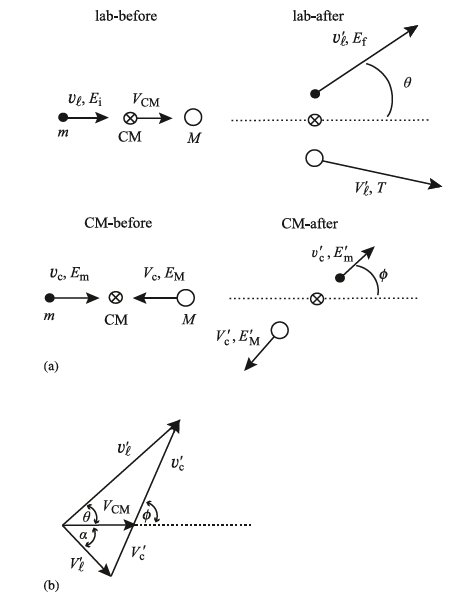
\includegraphics[width=0.8\linewidth]{triangles_GWas}
	\caption{Relationship between angles in CM and laboratory frame. (reference Gary Was book)}
	\label{fig:triangle}
\end{figure}

\begin{equation}
	\theta_L = \frac{1}{2} (\pi - \theta_C)
\label{eq:theta_relation}
\end{equation}

Let's define the cosine of the incident and scattered angles in the CM frame as $\mu_C$:

\begin{equation}
	\mu_C = \cos \theta_C
\end{equation}

And respectively, in the laboratory frame:

\begin{equation}
	\mu_L = \cos \theta_L
\end{equation}

Using Equation \ref{eq:theta_relation}, an expression for $\mu_L$ can be derived in terms of $\theta_C$ and $\mu_C$:

\begin{equation}
	\mu_L = \sin \left(\frac{\theta_C}{2}\right)
\end{equation}

\begin{equation}
	\mu_L = \sqrt{1 - \frac{\mu_C}{2}}
\end{equation}

Defining a mass fraction $\gamma$:

\begin{equation}
	\gamma = \frac{4 A}{(A+1)^2}
\end{equation}

The maximum transferred energy to the recoil atom can be written as:

\begin{equation}
	T = \frac{\gamma}{2} E_i (1-\mu_C)
\end{equation}

Working it backwards and solving for $\mu_C$

\begin{equation}
	\mu_C = 1 - \frac{2 T}{\gamma E}
	\label{eq:muc}
\end{equation}

For the elastic scattering, we have many variables describing the behavior of the collision. However, we only need two variables to define it, because the others will be given by the relationships described above.

%**********************************************************************************************************************************************************************************************%
\section{Recoil Production Rate Model Formulation}

The approach chosen in this project was to choose a neutron incident energy and the energy transferred to the recoil atom in order to define the elastic collision and we formulated our model accordingly. Recalling that we are interested in the production rate of recoil atoms, in order to quantify further radiation damage, we derived an approximate equation from the recoil production rate equation below:

\begin{equation}
	R(E \rightarrow T,\hat{\Omega}_T) = N_n  \int\limits_{4\pi} d \hat{\Omega}_r \int\limits_0^\infty dE_i \ \sigma_{s}(E_i \rightarrow T, \hat{\Omega}_i \rightarrow \hat{\Omega}_v) \psi(E_i, \hat{\Omega}_i)
\label{eq:rate}
\end{equation}

Where $N_n$ is the number density of fissile nuclei, $E_i$ is the incident neutron energy, T is the energy transferred to the recoil atom, $\hat{\Omega}_i$ is the incident neutron direction, $\hat{\Omega}_v$ is the scattered neutron direction, $\psi$ is the incident angular neutron flux. 

We can rewrite the elastic microscopic cross section as: $\sigma_{s}(E_i \rightarrow T, \hat{\Omega}_i \rightarrow \hat{\Omega}_v) = \sigma_{s}(E_i \rightarrow T, \hat{\Omega}_i \cdot \hat{\Omega}_v)$ because it is only dependent on the cosine between these two angles, not themselves (reference E.E. Lewis). This dot product is equal to the cosine of their angle in the laboratory frame. 

According to the Legendre polynomials properties, one can write:

\begin{equation}
	\int\limits_{-1}^1 dx P_l(x) P_{l'}(x) = \frac{2}{2l +1} \delta_{ll'}
\end{equation}

We can use Legendre polynomials to a different interval other than (-1,1) by shifting them. Basically we scale our variable to new the interval and use the regular Legendre polynomials. We are using the nomenclature $\tilde P_l(x)$ to refer to a Legendre Polynomial that uses a scaled interval and variable. The delta function $\delta_{ll'}$ ensures that this equation is only valid inside that interval.

\begin{equation}
	\int\limits_{a}^{b} dx \tilde P_l(x) \tilde P_{l'}(x) = \frac{b - a}{2l +1} \delta_{ll'}
\end{equation}

In order to use the Legendre polynomials shifted to a different interval other than (-1,1), a scaled variable must be used. 

\begin{equation}
	\tilde P_l (x) = P_l \left( \frac{x - a}{b - a}\right)
\end{equation}

We can approximate the elastic cross section with an expansion using Legendre polynomials, in which we get rid of the dependence in $\mu_L$:

\begin{equation}
	\sigma_{s}(E_i \rightarrow T, \mu_L) = 
	\begin{cases}
    		\sum\limits_{l=0}^{L} \frac{(2l +1)}{\Delta \mu_L} \  \sigma_{sl} (E_i \rightarrow T) \ \tilde P_l (\mu_L), & {\mu_L}_{min} \leq {\mu_L} \leq {\mu_L}_{max} \\
    		0,              & \text{otherwise}
\end{cases}
\label{eq:xs_expansion}
\end{equation}

Where $\sigma_{sl} (E_i \rightarrow T)$ are the coefficients of this Legendre expansion.

From Equation \ref{eq:xs_expansion}, we multiply both sides by $\tilde P_{l'}(\mu_L)$ and integrate with relation to $\mu_L$:

\begin{align}
	\int\limits_{{\mu_L}_{min}}^{{\mu_L}_{max}} d\mu_L \tilde P_{l'}(\mu_L) \sigma_{s}(E_i \rightarrow T, \mu_L)  &= \sum_{l =0}^{L} \frac{2l+1}{\Delta \mu_L} \sigma_{sl}(E_i \rightarrow T) \int\limits_{{\mu_L}_{min}}^{{\mu_L}_{max}} d\mu_L \tilde P_l(\mu_L) \tilde P_{l'}(\mu_L) \\
	\int\limits_{{\mu_L}_{min}}^{{\mu_L}_{max}} d\mu_L \tilde P_{l'}(\mu_L) \sigma_{s}(E_i \rightarrow T, \mu_L) &= \frac{2l'+1}{\Delta \mu_L} \frac{\Delta \mu_L}{2l'+1} \sigma_{sl}(E_i \rightarrow T)
\end{align}

Solving for the scattering cross section coefficients, we get:

\begin{equation}
	\sigma_{sl}(E_i \rightarrow T)= \int\limits_{{\mu_L}_{min}}^{{\mu_L}_{max}} d\mu_L \tilde P_{l'}(\mu_L) \sigma_{s}(E_i \rightarrow T, \mu_L)
\end{equation}

We need to approximate the scattering cross section inside this integral. 

\begin{equation}
	\phi_{lm}(E_i) \approx \xi (E_i)
\end{equation}


Average Cross section over group g

\begin{equation}
	\sigma_{slg}(T) \approx \frac{\int\limits_{{E}_{g+1}}^{E_g} d E_i \ \sigma_{s}(E_i \rightarrow T, \mu_L) \ \xi (E_i)}{\int\limits_{{E}_{g+1}}^{E_g} d E_i \ \xi (E_i) }
\end{equation}

Average over neutron group g

\begin{equation}
	\xi_g \equiv \int\limits_{{E}_{g+1}}^{E_g} d E_i \ \xi (E_i) 
\end{equation}

We can separate the cross section:

\begin{equation}
	\sigma_s (E_i \rightarrow T, \mu_L) = \sigma_s(E_i) \ f(E_i \rightarrow T, \mu_C)
\end{equation}

Where f is the scattering law. The scattering law is dependent on the incident neutron energy and the cosine of recoil angle in the CM frame. 

In order to get the recoil cross section from group g to energy bin t we need to also integrate of interval t. These are actually coefficients for Legendre expansion. 

\begin{equation}
	{\sigma}_{sl}^{g \rightarrow t} = \frac{1}{\xi_g}  \int\limits_{{T}_{t+1}}^{T_t} d T \int\limits_{E_{g+1}}^{E_g} dE_i \ \xi (E_i) \  \sigma_s (E_i)  \ \tilde P_l \left( \mu_L\right) \ f(E_i \rightarrow T, \mu_C) \ \delta_{ll'}
	\label{eq:xs_coeff}
\end{equation}

Substituting this to the Rate Equation (\ref{eq:rate}), we have: 

\begin{equation}
	R^{g \rightarrow t} (\hat{\Omega}_T) = \sum\limits_{g = 1}^{G}  \sum\limits_{l = 0}^{L} (2 l + 1) N_n {\sigma}_{sl}^{g \rightarrow t} \int\limits_{4\pi} d \hat{\Omega}_r \  \psi(\hat{\Omega}_i) \tilde P_l (\mu_L) H(\mu_L)
	\label{eq:ratefinal}
\end{equation}

Where 

\begin{equation}
	H(x) = 
	\begin{cases}
	1 ,&  x_{min} \leq x \leq x_{max} \\
	0 ,& \text{otherwise}
	\end{cases}
\end{equation}

%**********************************************************************************************************************************************************************************************%
\section{Numerical Implementation}

Firstly we implemented a recoil cross section calculator in MAGPIE, which is based on the MOOSE framework. This object takes as input: 

\begin{itemize}
 	\item isotope [a.m.u.]
	 \item neutron energy group boundaries [eV]
	 \item recoil energy bin boundaries [eV]
	 \item neutron spectrum 
	 \item neutron elastic cross section data [barn]
\end{itemize}

It returns as output a csv file with recoil cross sections coefficients ${\sigma}_{sl}^{g \rightarrow t}$ of the expansion in Legendre polynomials. This file can be postprocessed to calculate the overall sum in Legendre which will return the proper values of cross section according to Equation \ref{eq:xs_expansion}. The model takes Equation \ref{eq:xs_coeff} and calculates the integrals in $E_i$ and $T$ using a Gaussian quadrature rule as follows:

\begin{equation}
	{\sigma}_{sl}^{g \rightarrow t} = \frac{1}{\xi_g}  \sum\limits_{E_{g+1}}^{E_g}  \sum\limits_{{T}_{t+1}}^{T_t} \xi (E_{qp}) \  \sigma_s (E_{qp})  \ \tilde P_l \left( \mu_L\right) \ 	f(\mu_C) \ w_{E_{qp}} \ w_{T_{qp}}
	\label{eq:xs_num}
\end{equation}

We loop through all the neutron energy groups and recoil energy bins. For all the quadrature points inside these two intervals, we calculate the contribution for the cross section coefficient in which $\mu_C$ is given by the Equation \ref{eq:muc}. 


%**********************************************************************************************************************************************************************************************%
\section{Verification}

We compared the behavior of the elastic cross section with a simplified analytical solution for equation \ref{eq:xs_coeff} using constant parameters and Legendre order n = 0. The result is shown on Figure \ref{fig:analytical} and it behaved like expected. 

Figure \ref{fig:legendre7} shows the behavior of the recoil elastic cross section against the flight angle cosine. It is expected that recoils with greater energy will travel with smaller angles and therefore cosines closer to 1. Recoils with lower energies, which have angles closer to 90 degrees and cosines closer to zero. We can see the different behaviors according to the average recoil group energy in the same figure.

For the Legendre expansion, we did a very simple case with A = 1 and constant parameters (neutron spectrum, neutron elastic cross section, scattering law, etc). A good result was obtained with Legendre order n = 7. However, a drastic change in behavior is observed with n =8. This is because the order is too high and it is trying to converge, nonetheless the right behavior is not captured. This might be fixed with a higher order for the Gaussian quadrature integration rule. Figure \ref{fig:legendre8} shows the convergence issues with the Legendre expansion. 

\begin{figure}
	\centering
	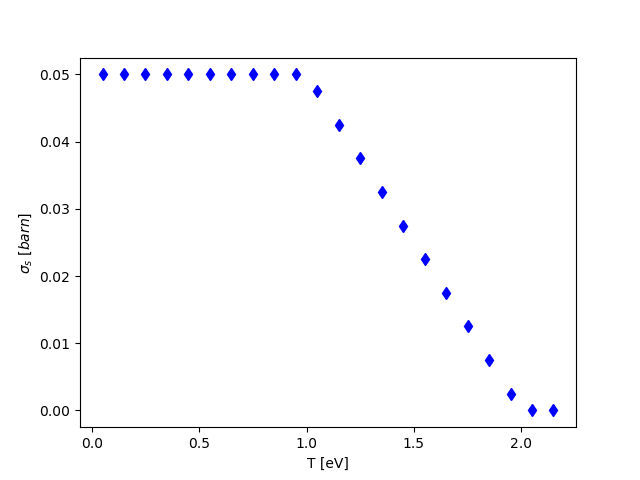
\includegraphics[width=0.5\linewidth]{erxs_analytical}
	\caption{Analytical comparison of the cross section coefficients }
	\label{fig:analytical}
\end{figure}

\begin{figure}
	\begin{subfigure}[h]{0.5\linewidth}
		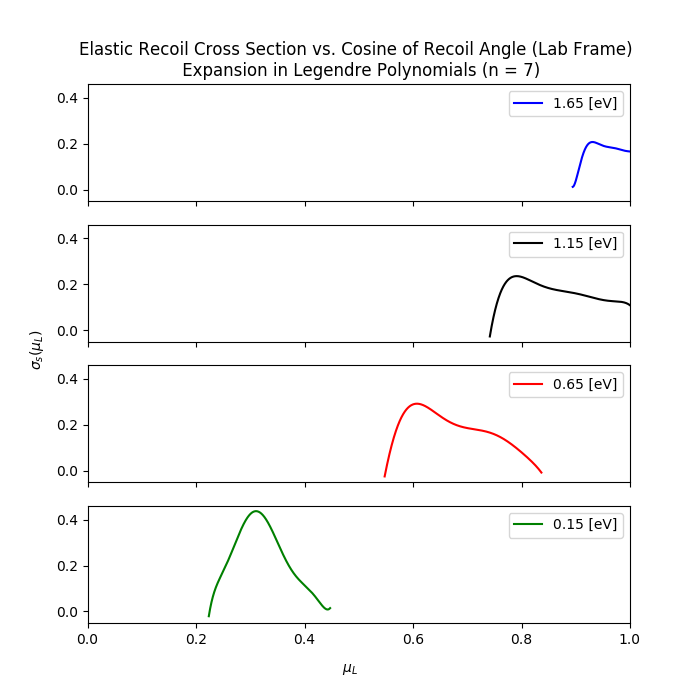
\includegraphics[width=\linewidth]{H_simple_plot_l7}
		\caption{n = 7}
		\label{fig:legendre7}
	\end{subfigure}
	\hfill
	\begin{subfigure}[h]{0.5\linewidth}
		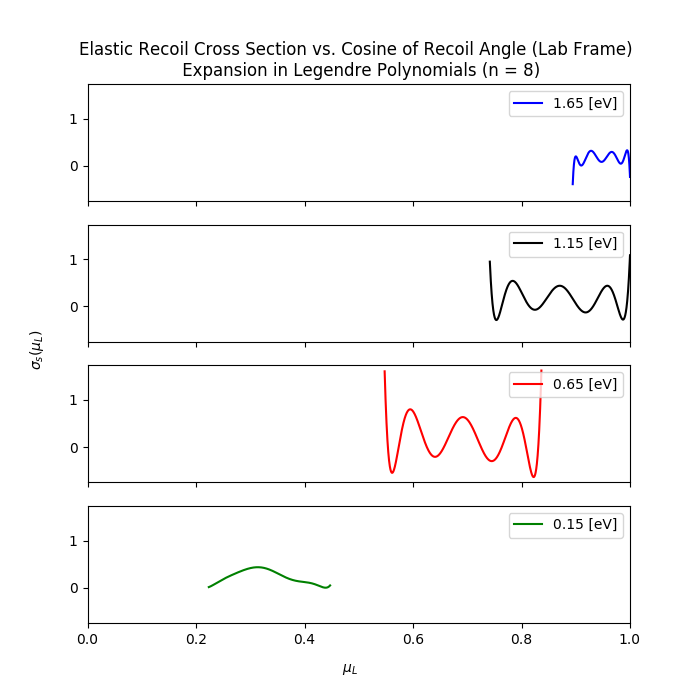
\includegraphics[width=\linewidth]{H_simple_plot_l8}
		\caption{n = 8}
		\label{fig:legendre8}
	\end{subfigure}%
	\caption{Behavior of the cross section for different orders for the Legendre Polynomials expansion. Figure \ref{fig:legendre7} shows the expansion with order n = 7 and 		Figure \ref{fig:legendre8}, n = 8. }
	\label{fig:legendre}
\end{figure}

%\section*{References}

%\bibliography{mybibfile}

\end{document}